% ============================
% TP Report – Simple Two-Column Template
% ============================
\documentclass[10pt,a4paper,twocolumn]{article}

% ---- Encoding & typography (simple, portable) ----
\usepackage[utf8]{inputenc}
\usepackage[T1]{fontenc}
\usepackage{lmodern}
\usepackage{microtype}
\usepackage{amsmath}

% ---- Layout ----
\usepackage{geometry}
\geometry{
  left=1.4cm, right=1.4cm,
  top=1.5cm, bottom=1.5cm,
  columnsep=0.55cm
}
\usepackage{balance} % balances the final page columns

% ---- Graphics ----
\usepackage{graphicx}
\usepackage[font=small,labelfont=bf]{caption}

% ---- Useful tweaks (optional) ----
\setlength{\parskip}{0pt}   % compact paragraphs
\setlength{\parindent}{1em} % classic indent; comment out if you prefer no indents

% ============================
%            Title
% ============================
\title{\vspace{-6mm}\textbf{TP2: Identification de la dynamique d'un robot manipulateur à deux axes
Linéaire}}
\author{Léo Sabatié, Esteban Peregrina \quad (Groupe 2, ROB5) \\ 
Enseignant: Mahdi Khoramshahi \quad École: Polytech Sorbonne}
\date{\today}

\begin{document}
\maketitle
% ============================
%           Sections
% ============================
\section{Étude théorique}
\subsection{Modèle dynamique avec un paramétrage relatif}

La méthode de Newton-Euler permet d'écrire le modèle dynamique 
d'un robot série à $N$ segments $S_i$.

À partir des torseurs cinématique et cinétique de chaque segment, 
ainsi que de leur accélération exprimée en leur centre de gravité. \\
On considère alors un système $\Sigma = \{\}$. Pour $i$ allant de
$1$ à $N$, on applique (en fonction de la liaison courante) soit 
le théorème du moment dynamique soit le théorème de la résultante dynamique, 
au système $\Sigma = \Sigma \cup \{S_i\}$. En projetant sur l'axe de l'articulation 
considérée, on aboutit aux équations dynamique du système qui peuvent être mis
sous la forme matricielle suivante :
\begin{equation}
  [A(q)][\ddot{q}] + [B(q,\dot{q})]+[C(q)][\dot{q}]+g[g(q)] = [\Gamma]
\label{eq:modele_general}
\end{equation}

En l'occurence, le robot étudié n'est ici formé que de deux segments en liaison pivot.
L'application du théorème du moment dynamique au centre de la liason et projeté sur l'axe
du pivot donne : 
\begin{equation}
  \begin{aligned}
    \begin{pmatrix}
      \Gamma_1 \\
      \Gamma_2
    \end{pmatrix}
    &=
    \underbrace{
      \begin{pmatrix}
        I'_1 + I'_2 + m_2l_1^2 + 2h\cos(\theta_2) & I'_2 + h\cos(\theta_2) \\
        I'_2 + h\cos(\theta_2) & I'_2
      \end{pmatrix}
    }_{A(\mathbf{q})}
    \begin{pmatrix}
      \ddot{\theta}_1 \\
      \ddot{\theta}_2
    \end{pmatrix}
    \\[0.5em]
    &\quad+
    \underbrace{
      \begin{pmatrix}
        -2h\sin(\theta_2) \\
        0
      \end{pmatrix}
    }_{B(\mathbf{q})}
    \dot{\theta}_1\dot{\theta}_2
    \\[0.5em]
    &\quad+
    \underbrace{
      \begin{pmatrix}
        0 & -h\sin(\theta_2) \\
        h\sin(\theta_2) & 0
      \end{pmatrix}
    }_{C(\mathbf{q})}
    \begin{pmatrix}
      \dot{\theta}_1 \\
      \dot{\theta}_2
    \end{pmatrix}
    \\[0.5em]
    &\quad+
    g\,
    \underbrace{
      \begin{pmatrix}
        m_2\lambda_2\cos(\theta_1+\theta_2) + m_1\lambda_1\cos(\theta_1) \\
        m_2\lambda_2\cos(\theta_1+\theta_2)
      \end{pmatrix}
    }_{\mathbf{g}(\mathbf{q})}.
  \end{aligned}
\label{eq:modele_relatif}
\end{equation}

Les paramètres regroupés dans ce modèle sont définis par :
\begin{equation}
  \begin{aligned}
    I'_1 &= I_1 + m_1\lambda_1^2,\\
    I'_2 &= I_2 + m_2\lambda_2^2,\\
    h &= m_2\lambda_2l_1.
  \end{aligned}
\label{eq:parametres_relatifs}
\end{equation}

\subsection{Réécriture avec un paramétrage absolu}

Jusqu'à présent, le modèle dynamique a été exprimé à l'aide d'un paramétrage relatif des articulations. 
Dans la suite, nous adoptons un paramétrage absolu, dans lequel $\theta'_1$ et $\theta'_2$ 
représentent directement les orientations absolues des deux bras. Ce changement de coordonnées 
nécessite de reparamétrer à la fois les variables articulaires et les couples associés.

La relation entre les coordonnées relatives $\mathbf{q}$ et les coordonnées absolues $\mathbf{q'}$ s'écrit :
\begin{equation}
  \begin{pmatrix}
    \theta'_1\\
    \theta'_2
  \end{pmatrix}
  =
  \underbrace{
    \begin{pmatrix}
    1 & 0\\
    1 & 1
    \end{pmatrix}
  }_{E}
  \begin{pmatrix}
    \theta_1\\
    \theta_2
  \end{pmatrix}.
\label{eq:transformation_q}
\end{equation}

On en déduit les relations inverses :
\begin{equation}
  \begin{pmatrix}
    \theta_1\\
    \theta_2
  \end{pmatrix}
  =
  E^{-1}
  \begin{pmatrix}
    \theta'_1\\
    \theta'_2
  \end{pmatrix},
  \qquad
  E^{-1}
  =
  \begin{pmatrix}
    1 & 0\\
    -1 & 1
  \end{pmatrix}.
\label{eq:transformation_q_inverse}
\end{equation}

Les couples doivent également être reparamétrés. La relation entre les couples relatifs 
et absolus est donnée par :
\begin{equation}
  \begin{aligned}
    \begin{pmatrix}
      \Gamma'_1\\
      \Gamma'_2
    \end{pmatrix}
    &=
    E^{-T}
    \begin{pmatrix}
      \Gamma_1\\
      \Gamma_2
    \end{pmatrix}, \\
    \text{avec} \quad E^{-T}
    &=
    E^{T} \times E^{-1}
    =
    \begin{pmatrix}
      1 & -1\\
      0 & 1
    \end{pmatrix}.
  \end{aligned}
\label{eq:transformation_gamma}
\end{equation}

On peut utiliser ces relations pour trouver l'expression de $\theta_1', \theta_2', \Gamma_1', \Gamma_2',$
en fonction des paramètres relatifs. 
En injectant ces expressions dans le modèle dynamique \eqref{eq:modele_relatif}, et après
après développement et regroupement des différents termes, le modèle dynamique exprimé dans 
les coordonnées absolues prend finalement la forme :
\begin{equation}
  \begin{aligned}
    \begin{pmatrix}
      \Gamma'_1\\
      \Gamma'_2
    \end{pmatrix}
    &=
    \underbrace{
      \begin{pmatrix}
        I'_1 + m_2l_1^2 & h\cos(\theta'_2-\theta'_1) \\
        h\cos(\theta'_2-\theta'_1) & I'_2
      \end{pmatrix}
    }_{A'(\mathbf{q}')}
    \begin{pmatrix}
      \ddot{\theta}'_1 \\
      \ddot{\theta}'_2
    \end{pmatrix}
    \\[0.5em]
    &\quad+
    \underbrace{
      \begin{pmatrix}
        0 \\
        0
      \end{pmatrix}
    }_{B'(\mathbf{q}')}
    \dot{\theta}'_1\dot{\theta}'_2
    \\[0.5em]
    &\quad+
    \underbrace{
      \begin{pmatrix}
        0 & -h\sin(\theta'_2-\theta'_1) \\
        h\sin(\theta'_2-\theta'_1) & 0
      \end{pmatrix}
    }_{C'(\mathbf{q}')}
    \begin{pmatrix}
      \dot{\theta}'_1\\
      \dot{\theta}'_2
    \end{pmatrix}
    \\[0.5em]
    &\quad+
    g\,
    \underbrace{
      \begin{pmatrix}
        (m_2l_1+m_1\lambda_1)\cos(\theta'_1) \\
        m_2\lambda_2\cos(\theta'_2)
      \end{pmatrix}
    }_{\mathbf{g}'(\mathbf{q}')}.
  \end{aligned}
\label{eq:modele_absolu}
\end{equation}

On remarque notamment que, dans le paramétrage absolu, le terme
\[
B'(\mathbf{q}')\dot{\theta}'_1\dot{\theta}'_2
\]
est nul. Tous les termes dépendant des vitesses sont alors regroupés dans la matrice $C'(\mathbf{q}')$.

Le couple de gravité exercé sur l'axe 1 ne dépent plus de la position de l'axe 2 car la 
liaison pivot n'est plus actionnée. Cette dernière étant supposée parfaite, aucun effort
ne peut être transmis par l'axe 2. Le référentiel n'étant plus en rotation, les effets de Corriolis
(matrice $B'(q)$) sont nuls. Lorsque $cos(\theta_2' - \theta_1') = 0$, cela signifie que le bras est tendu
et l'inertie correspond à celle d'un axe simple, la symétrie annulant les produit d'inertie de la matrice
d'inertie.

\subsection{Intégration de la dynamique des actionneurs}
L'intégration de la dynamique des actionneurs se fait en remplaçant le membre de gauche de
\eqref{eq:modele_relatif} par le modèle fourni. Il faut développer l'équation matricielle puis rassembler
les termes $\ddot\theta$ dans la matrice d'inertie.

\subsection{Identification des frottements et des termes de gravité}
Afin d'identifier les paramètres de frottement et de gravité du système, on simplifie le modèle 
en faisant l'hypothèse que l'axe 1 est immobile et que l'axe 2 se déplace à vitesse constante.
Ainsi, on peut aboutir la relation linéaire suivante entre le couple du second reducteur  $\Gamma_1$ 
et nos paramètres $p$ : 

Afin de résoudre l'équation sur MATLAB, il faudra réaliser un minimum de $n_p = 4$ mesures de $Y$ notées 
$Y_k$ pour $k \in \{1,2,3,4\}$ et qu'on concatenera dans une matrice carré (donc inversible). Le terme
de gauche sera construit par concaténation des entrées ayant produites les mesures (seul le courant $i_2$ 
varie). Davantage de mesures permettent d'obtenir un système surdéterminé pour affiner les résultats.

Pour l'axe 1, on supposera que l'axe 1 se déplace à vitesse constante, et on prendra $\theta_1', \theta_2'$
tel que, à tout instant, $cos(\theta_2' - \theta_1') = 0$. On procède ensuite de la même 
façon qu'avec l'axe 2.


\subsection{Identification des autres termes du modèle dynamique}
En développant l'équation (5) et en rassemblant les paramètres dynamique restant, on aboutit à l'équation
suivante :  

\section{Manipulations}
\subsection{Identification des frottements et de la gravité sur l'axe 2}

\begin{figure}[!h]
  \centering
  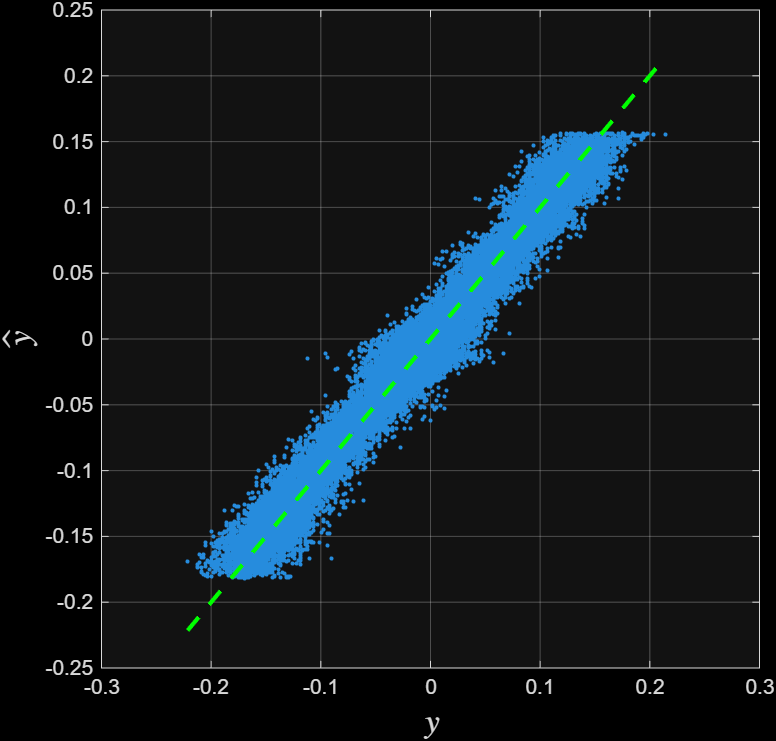
\includegraphics[width=0.30\textwidth]{Comparaison_valeurs_mesurées_estimées.png}
  \caption{Comparaison entre les valeurs mesurées et les valeurs estimées par le modèle avec les données brutes ($i_2$ et $q_p$)}
  \label{fig:summary}
\end{figure}

\begin{figure}[!h]
  \centering
  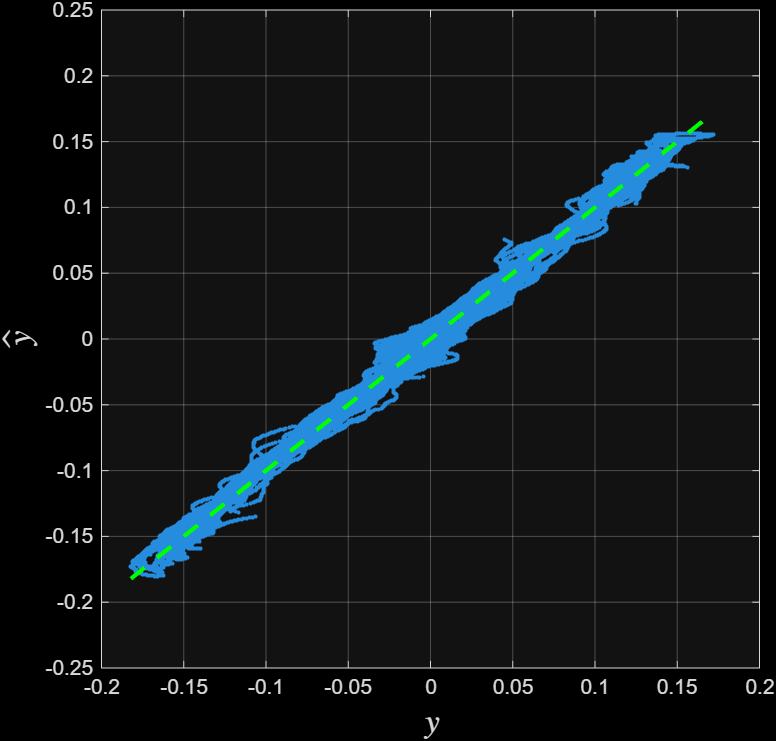
\includegraphics[width=0.30\textwidth]{Comparaison_valeurs_mesurées_estimées_filtre.png}
  \caption{Comparaison entre les valeurs mesurées et les valeurs estimées par le modèle avec les données filtrées ($i_{2,fil}$ et $q_{p,fil}$).}
  \label{fig:summary}
\end{figure}

Lorsque nous utilisons les données brutes pour estimer les paramètres, on peut observer une plus grande dispertion des points autour de la diagonale
Cette dispersion traduit des écarts plus importants entre les valeurs mesurées et les valeurs estimées par le modèle, notamment en raison du bruit présent dans les mesures. Après filtrage des données, les points se rapprochent davantage de la droite ($y=\hat{y}$), ce qui indique une diminution des écarts entre les mesures et les estimations et donc une meilleure concordance avec le modèle identifié.



Lorsque l'on regroupe nos mesures, on aboutit à l'équation matricielle suivante :
\begin{equation}
  \begin{array}{ccl}
    Y = Ap
  \end{array}
\end{equation}
où $p$ est le vecteur des neufs paramètres matériels, $A$ la matrice de régression concaténée, 
et $Y$ la matrice des sorties measurées concaténées.



Les données obtenues sont donc utilisées pour construire la matrice $A$.

\subsection{Identification des frootements et de la gravité sur l'axe 1}
\noindent\textbf{Identification des paramètres.} La résolution de l'équation $(1)$ sous MATLAB conduit à l'identification des paramètres.
Le choix des mesures utilisées est important : si les mesures sont trop
similaires, les lignes de $A$ deviennent proches et le problème est mal
conditionné. Il est donc nécessaire de disposer de mesures suffisamment
riches afin d'obtenir une identification fiable.

Ainsi, le calcul du conditionnement et du rang de $A$ permettent
d'évaluer la qualité du problème d'identification.

% ============================
% Quantification et filtrage
% ============================
\subsection{Identification des autres termes du modèle dynamique}
\noindent\textbf{Quantification et filtrage.} Les positions, vitesses et accélérations simulées sont ensuite quantifiées
avec les résolutions imposées dans le TP. Cette opération introduit une
erreur sur les mesures, qui se répercute directement sur l'identification.

Un filtrage des données quantifiées est également étudié. Nous avons
constaté que le filtrage ne conduit pas nécessairement à une meilleure
identification : en supprimant certaines composantes du signal, il peut
également supprimer des informations utiles à l'estimation des paramètres.
Le choix du paramètre du filtre doit donc être réalisé en comparant les
erreurs d'identification.

% ============================
% Etude complémentaire
% ============================
\noindent\textbf{Étude complémentaire.} Lorsque $k_1$ et $b_1$ deviennent très grands, les deux premières masses
sont fortement couplées. On obtient alors approximativement
\[
\alpha\simeq\beta,\qquad
\dot{\alpha}\simeq\dot{\beta},\qquad
\ddot{\alpha}\simeq\ddot{\beta}.
\]

Les paramètres $k_1$ et $b_1$ ne peuvent alors plus être correctement
identifiés. Le modèle est donc réduit afin de ne conserver que les
paramètres identifiables :
\[
p_r =
[k_0,\ k_2,\ b_0,\ b_2,\ m_1+m_2,\ m_3]^T.
\]

Pour ce modèle réduit, nous obtenons $\mathrm{cond}(A)=98$.
Les erreurs obtenues sont notamment de $0.12\%$ pour $k_0$,
$1.22\%$ pour $b_0$, $4.30\%$ pour $b_2$ et $4.84\%$ pour $m_3$.
L'erreur sur $m_1+m_2$ reste cependant plus importante, avec $33.35\%$.

% ============================
% Conclusion
% ============================
\section*{Conclusion}
???

\balance
\end{document}